\documentclass[12pt]{article}
\usepackage{mathrsfs,hyperref,amsmath,amsfonts,fullpage,color,tikz}
\newcommand{\be}{\begin{equation}}
\newcommand{\ee}{\end{equation}}
\newcommand{\bh}{\bar{h}}
\usepackage{enumitem}
\newcounter{quesno}
\newcommand{\ques}[1]{\vspace{2em}\stepcounter{quesno}
\noindent{\bf Question \thequesno.} \emph{(#1 points)}\\
}
\begin{document}
\begin{center}
{\bf\Large General Relativity --- Final Examination}\\[0.5em]
{\bf\large Answers}
\end{center}
\hrule

\ques{2}
Under $x^\mu\to x'^\mu(x)$ the Riemann tensor transforms as a $(1,3)$ tensor:
\be
R'^\mu{}_{\nu\rho\sigma}=\frac{\partial x'^\mu}{\partial x^\alpha}\frac{\partial x^\beta}{\partial x'^\nu}\frac{\partial x^\gamma}{\partial x'^\rho}\frac{\partial x^\delta}{\partial x'^\sigma}R^\alpha{}_{\beta\gamma\delta}.
\ee
Contracting the first and third indices,
\begin{align}
R'_{\nu\sigma}=R'^\rho{}_{\nu\rho\sigma}
&=\frac{\partial x'^\rho}{\partial x^\alpha}\frac{\partial x^\gamma}{\partial x'^\rho}\frac{\partial x^\beta}{\partial x'^\nu}\frac{\partial x^\delta}{\partial x'^\sigma}R^\alpha{}_{\beta\gamma\delta}.
\end{align}
By the chain rule $\frac{\partial x'^\rho}{\partial x^\alpha}\frac{\partial x^\gamma}{\partial x'^\rho}=\frac{\partial x^\gamma}{\partial x^\alpha}=\delta^\gamma_\alpha$, so
\be
R'_{\nu\sigma}=\frac{\partial x^\beta}{\partial x'^\nu}\frac{\partial x^\delta}{\partial x'^\sigma}R^\alpha{}_{\beta\alpha\delta}=\frac{\partial x^\beta}{\partial x'^\nu}\frac{\partial x^\delta}{\partial x'^\sigma}R_{\beta\delta},
\ee
which is the transformation law of a $(0,2)$ tensor.

\ques{3}
Convention: $\nabla_\mu V^\rho=\partial_\mu V^\rho+\Gamma_{\mu\nu}{}^\rho V^\nu$.

\begin{enumerate}[label=\alph*)]
\item Torsion is $\hat T_{\mu\nu}{}^\rho=\hat\Gamma_{\mu\nu}{}^\rho-\hat\Gamma_{\nu\mu}{}^\rho=0+\frac{1}{12}g^{\rho\sigma}(H_{\mu\nu\sigma}-H_{\nu\mu\sigma})=\frac16 g^{\rho\sigma}H_{\mu\nu\sigma}$, since $\Gamma$ is symmetric. This is non-zero unless $H=0$, so the connection is \emph{not} torsion-free.

Metric compatibility:
\begin{align}
\hat\nabla_\mu g_{\nu\rho}&=\partial_\mu g_{\nu\rho}-\hat\Gamma_{\mu\nu}{}^\sigma g_{\sigma\rho}-\hat\Gamma_{\mu\rho}{}^\sigma g_{\nu\sigma}\\
&=\nabla_\mu g_{\nu\rho}-\tfrac1{12}\left(H_{\mu\nu\rho}+H_{\mu\rho\nu}\right)=0-0=0,
\end{align}
using $\nabla g=0$ for Levi-Civita and antisymmetry of $H$. So it \emph{is} metric compatible.

\item Geodesics of $\hat\Gamma$: $\ddot x^\rho+\hat\Gamma_{\mu\nu}{}^\rho\dot x^\mu\dot x^\nu=0$. Then
\be
\ddot x^\rho+\Gamma_{\mu\nu}{}^\rho\dot x^\mu\dot x^\nu+\tfrac1{12}g^{\rho\sigma}H_{\mu\nu\sigma}\dot x^\mu\dot x^\nu=0,
\ee
and the last term vanishes because $H_{\mu\nu\sigma}$ is antisymmetric in $\mu\nu$ while $\dot x^\mu\dot x^\nu$ is symmetric. The equation is the Levi-Civita geodesic equation.
\end{enumerate}

\ques{4}
\begin{enumerate}[label=\alph*)]
\item The metric components are singular at $r=0$ and $r=2GM$ (also the usual polar-coordinate artefact at $\theta=0,\pi$). The surface $r=2GM$ is only a \emph{coordinate} singularity (the event horizon): curvature invariants are finite there, e.g.\ the Kretschmann scalar $R_{\mu\nu\rho\sigma}R^{\mu\nu\rho\sigma}=48G^2M^2/r^6$, and a freely falling observer crosses it in finite proper time, feeling nothing special locally. At $r=0$ the curvature invariant diverges: this is a genuine \emph{curvature} singularity, where tidal forces become infinite and one is destroyed in finite proper time. This is the one to worry about (the horizon, however, means you cannot return or signal out).
\item Differentiating, $dv=dt+dr\left(1+\frac{2GM}{r-2GM}\right)=dt+\frac{dr}{f}$, so $dt=dv-dr/f$. Then
\be
-f\,dt^2=-f\,dv^2+2\,dv\,dr-\frac{dr^2}{f},
\ee
and the $dr^2/f$ terms cancel:
\be
ds^2=-f(r)\,dv^2+2\,dv\,dr+r^2d\theta^2+r^2\sin^2\theta\,d\phi^2 .
\ee
The metric components are smooth at $r=2GM$ and the determinant is $-r^4\sin^2\theta$, non-zero there, so the metric is regular and invertible and extends smoothly to $r<2GM$: $r=2GM$ was a coordinate artefact. At $r=0$ the metric is still singular and no coordinate change removes this, as the curvature invariant diverges; this confirms the answer to a).
\end{enumerate}

\ques{5}
\begin{enumerate}[label=\alph*)]
\item The metric has the FRW form $ds^2=-dt^2+a(t)^2d\Omega_3^2$ with a closed ($k=+1$) spatial slice: it is homogeneous and isotropic, as observed on large scales, and it solves Einstein's equations with a positive cosmological constant (dark energy, $\Lambda=3/L^2$), which describes accelerated expansion. The scale factor is $a(t)=L\cosh(t/L)$, contracting for $t<0$, with minimum $L$ at $t=0$, then expanding, approaching $\tfrac L2e^{t/L}$ (exponential expansion) at late times.
\item If $g=\Omega^2\bar g$ with $\Omega$ smooth and positive, then a curve with tangent $k^\mu$ has $g_{\mu\nu}k^\mu k^\nu=\Omega^2\bar g_{\mu\nu}k^\mu k^\nu$, which has the same sign. So timelike, null and spacelike vectors and curves coincide for both metrics; the light cones, and hence causal relations, are identical. Null geodesics are also the same (as unparametrised curves).
\item From $\cosh(t/L)=1/\cos\eta$: $\sinh(t/L)=\tan\eta$, and differentiating, $\frac1L\sinh(t/L)\,dt=\frac{\sin\eta}{\cos^2\eta}d\eta$, so $dt=\frac{L\,d\eta}{\cos\eta}$. Then
\be
ds^2=\frac{L^2}{\cos^2\eta}\left(-d\eta^2+d\chi^2+\sin^2\chi\,d\Omega_2^2\right),\qquad \eta\in(-\tfrac\pi2,\tfrac\pi2).
\ee
This is conformal to a finite piece of the Einstein static universe, with conformal factor $\Omega=L/\cos\eta$. Radial null rays satisfy $\eta=\pm\chi+$const, i.e.\ 45$^\circ$ lines. The Penrose diagram is a square: $\chi=0$ and $\chi=\pi$ (the north and south poles) are vertical lines on the left and right (each point is a 2-sphere, except at the poles), $\eta=-\pi/2$ is the spacelike past infinity $\mathscr I^-$ at the bottom, and $\eta=+\pi/2$ is the spacelike future infinity $\mathscr I^+$ at the top; the $t=0$ slice is $\eta=0$. An observer at the north pole can only see part of the space: its particle horizon and event horizon are the null lines from the corners.
\begin{center}
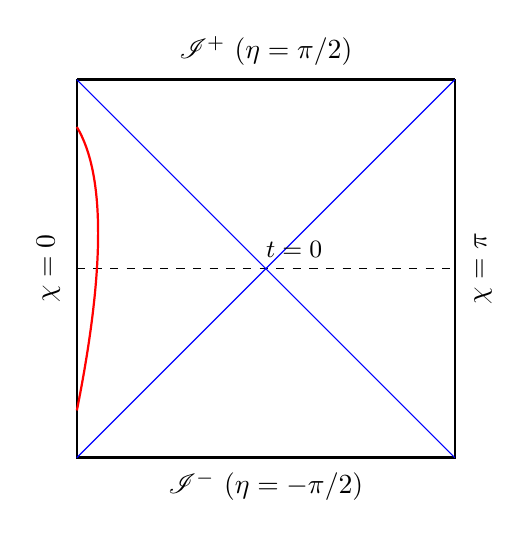
\begin{tikzpicture}[scale=1.2]
\draw[thick] (0,0)--(4,0)--(4,4)--(0,4)--cycle;
\draw[very thick] (0,4)--(4,4); \draw[very thick] (0,0)--(4,0);
\draw[dashed] (0,2)--(4,2);
\draw[blue] (0,0)--(4,4); \draw[blue] (4,0)--(0,4);
\node at (2,4.3) {$\mathscr I^+$ ($\eta=\pi/2$)};
\node at (2,-0.3) {$\mathscr I^-$ ($\eta=-\pi/2$)};
\node[rotate=90] at (-0.3,2) {$\chi=0$};
\node[rotate=90] at (4.3,2) {$\chi=\pi$};
\node at (2.3,2.2) {\small $t=0$};
\draw[red,thick] (0,0.5) .. controls (0.3,2) and (0.3,3) .. (0,3.5);
\end{tikzpicture}
\end{center}
\end{enumerate}

\ques{6}
\begin{enumerate}[label=\alph*)]
\item Under $x^\mu\to x^\mu+\xi^\mu$, $\bh_{\mu\nu}\to\bh_{\mu\nu}-\partial_\mu\xi_\nu-\partial_\nu\xi_\mu+\eta_{\mu\nu}\partial\cdot\xi$, so $\partial^\mu\bh_{\mu\nu}\to\partial^\mu\bh_{\mu\nu}-\Box\xi_\nu$. We can always choose $\xi$ with $\Box\xi_\nu=\partial^\mu\bh_{\mu\nu}$ and thereby impose the Lorenz (de Donder) gauge $\partial^\mu\bh_{\mu\nu}=0$. The second and third terms of the equation then vanish, leaving $\Box\bh_{\mu\nu}=-16\pi G T_{\mu\nu}$. In vacuum, $(-\partial_t^2+\nabla^2)\bh_{\mu\nu}=0$: a wave equation with solutions $\bh_{\mu\nu}(t-z)$ travelling at the speed of light, i.e.\ gravitational waves.
\item For freely falling particles initially at rest, the geodesic equation gives $\ddot x^i=-\Gamma^i_{00}=-\frac12(2\partial_0h_{i0}-\partial_ih_{00})=0$ at linear order, since $h_{0\mu}=0$. So the particles remain at fixed coordinate positions. The proper distance at fixed $t$ between $(0,0,0)$ and $(L_x,0,0)$, with $h_{xx}=h_+(t-z)$ evaluated at $z=0$, is
\be
\Delta s=\int_0^{L_x}\sqrt{1+h_{+}(t)}\,dx\approx L_x\left(1+\tfrac12h_+(t)\right),
\ee
using $h_+\ll1$. For the particle at $(0,L_y,0)$, $h_{yy}=-h_+$ so
\be
\Delta s=\int_0^{L_y}\sqrt{1-h_{+}(t)}\,dy\approx L_y\left(1-\tfrac12h_+(t)\right).
\ee
The wave stretches distances along $x$ while squeezing along $y$, and vice versa half a cycle later.
\item Two bodies orbiting radiate gravitational waves (the time-varying mass quadrupole), at twice the orbital frequency, $f_{GW}=2f_{orb}$. The radiated energy is taken from the orbit, so the bodies spiral together.
\begin{itemize}
\item \emph{Inspiral}: the orbit shrinks slowly and quasi-circularly; as the separation decreases the orbital frequency increases, so both the frequency and amplitude of the signal increase with time (a ``chirp''). The amplitude is $h\sim (G\mathcal M)^{5/3}f^{2/3}/(c^4 d)$, where the chirp mass $\mathcal M$ controls the rate of increase of frequency and $d$ is the distance.
\item \emph{Merger}: when the bodies reach the innermost stable orbit and plunge together, the system is highly relativistic and non-linear (needs numerical relativity); the signal peaks in amplitude and frequency.
\item \emph{Ringdown}: the final merged object (a black hole) is initially deformed, and settles to a stationary Kerr black hole by radiating its distortion away as quasinormal modes: a damped sinusoid with constant frequency and exponentially decaying amplitude, whose frequency and decay time depend only on the final mass and spin.
\end{itemize}
\begin{center}
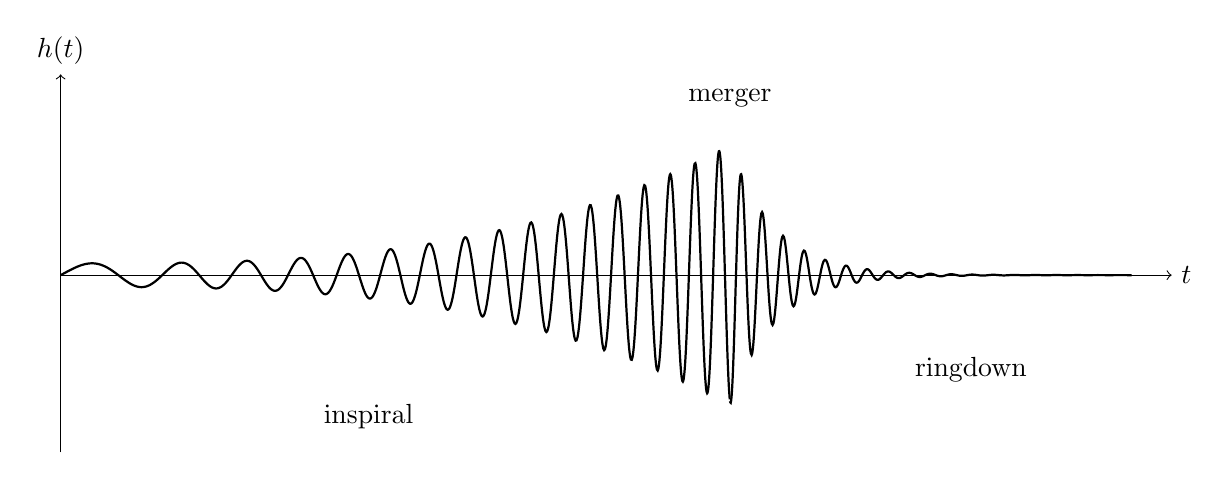
\begin{tikzpicture}[xscale=1.7,yscale=1.5]
\draw[->] (0,-1.5)--(0,1.7) node[above] {$h(t)$};
\draw[->] (0,0)--(8.3,0) node[right] {$t$};
\draw[thick,domain=0:5,samples=800,smooth] plot (\x,{(0.1+0.008*\x*\x*\x)*sin((6*\x+3*\x*\x) r)});
\draw[thick,domain=5:8,samples=500,smooth] plot (\x,{1.1*exp(-3*(\x-5))*sin((105+40*(\x-5)) r)});
\node at (2.3,-1.2) {inspiral}; \node at (5,1.5) {merger}; \node at (6.8,-0.8) {ringdown};
\end{tikzpicture}
\end{center}
The detector (LIGO) is a Michelson interferometer with two perpendicular arms (4\,km) with Fabry--Perot cavities. By b), a wave with $+$ polarisation incident along $z$ lengthens one arm while shortening the other, $\Delta L_x-\Delta L_y=L\,h_+(t)$, changing the interference of the two returning laser beams: the output photodiode signal is proportional to $h(t)$, with $h\sim10^{-21}$. The signal's features map onto the physics: the chirp rate gives the chirp mass, the amplitude gives distance, the merger frequency gives the total mass, and the ringdown frequency and damping time give the mass and spin of the remnant black hole.
\end{enumerate}
\end{document}
